\section{Results}
\label{sec:results}

The baseline estimate uses the labor-only informal sector, the statutory non-wage costs of formal employees and the available data from 1993Q2 to 2026Q2: the five aggregate growth rates, the level of the informality rate, including the ICML reconstruction of the labor market, and the value-added earnings ratio from 2007. The equal-technology estimate is reported as an upper bound and the estimate without earnings as a reference.

\subsection{Posterior and convergence}

Table~\ref{tab:posterior} reports the prior, the posterior median and 90\% interval, the ratio of posterior to prior standard deviation, and the convergence diagnostics. The largest rank-normalized $\hat R$ is 1.005, for $\theta$. The smallest bulk effective sample size is 1{,}718 and the smallest tail effective sample size 1{,}067, out of 320{,}000 retained draws; acceptance rates are between 0.23 and 0.30.

\begin{table}[H]
\centering
\caption{Prior and posterior distributions, baseline estimate (labor-only informal sector, statutory non-wage costs).}
\label{tab:posterior}
\scriptsize
\begin{tabular}{l l r c r r r}
\toprule
\textbf{Parameter} & \textbf{Prior (mean, sd)} & \textbf{Median} & \textbf{90\% interval} & \textbf{sd ratio} & $\hat R$ & \textbf{ESS} \\
\midrule
\tableinput{tables/posterior.tex}
\bottomrule
\end{tabular}
\end{table}

The steady-state informal share has a posterior median of 0.262 and a 90\% interval of 0.240--0.277; its posterior standard deviation is 12\% of the prior one, against 57\% when the earnings ratio is not observed (Figure~\ref{fig:prior-posterior}). As Section~\ref{sec:id-baseline} shows, this concentration owes part of its strength to the priors on the persistence of the shocks; the object identified by the data is the path of the share. The median earnings ratio is $R\approx0.31$: informal income per worker is about 31\% of the labor cost of a formal employee, and informal value added per worker, $(1-\alpha)R$, is about 20\% of formal value added per worker. The labor elasticity of informal production $\eta$ is not informed by the data (its posterior is the prior). The informal-productivity shock is persistent (0.92) and small (1.6\% per quarter), and the measurement error of the earnings ratio is 3.3\%. With formal employees in the denominator, the level shift of the earnings ratio in 2022 is small and not distinguishable from zero ($-0.035$, 90\% interval $-0.079$ to $0.009$).

\begin{figure}[H]
\centering
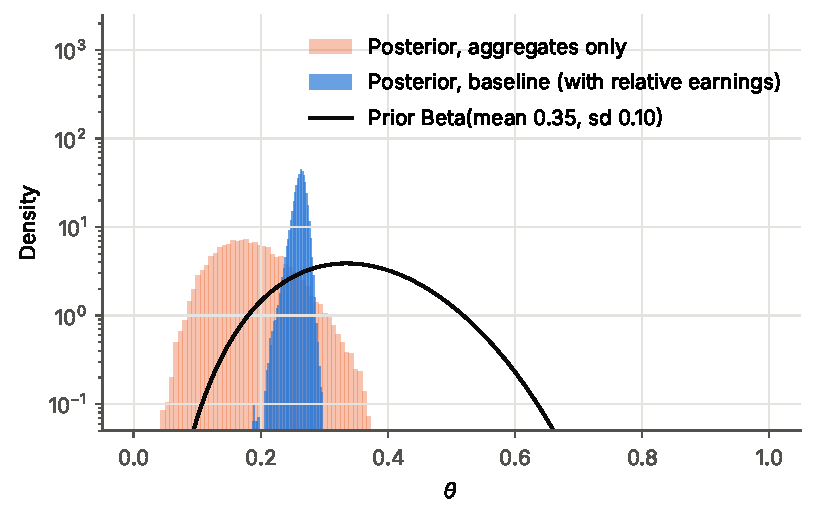
\includegraphics[width=0.75\textwidth]{fig_prior_posterior.pdf}
\caption{Prior and posteriors of the steady-state informal share $\theta$: baseline with the earnings observable and estimate with aggregates only (logarithmic density scale).}
\label{fig:prior-posterior}
\end{figure}

\subsection{Fit}

Table~\ref{tab:fit} compares the root mean squared one-step-ahead prediction error of the model with the standard deviation of each observable and with the error of a univariate first-order autoregression. Because quarterly growth rates have almost no persistence, the relevant benchmark is the autoregression. The model is within about three percent of it for GDP, consumption and employment, and improves on it for government consumption. The informality rate, now observed in levels, is predicted with an error of 15\% of its standard deviation, close to that of the autoregression.

\begin{table}[H]
\centering
\caption{One-step-ahead prediction, baseline estimate (pandemic quarters excluded).}
\label{tab:fit}
\footnotesize
\begin{tabular}{l r r r r}
\toprule
\textbf{Observable} & \textbf{sd} & \textbf{Autocorrelation} & \textbf{RMSE/sd, model} & \textbf{RMSE/sd, AR(1)} \\
\midrule
\tableinput{tables/fit.tex}
\bottomrule
\end{tabular}
\end{table}

\subsection{What drives informality}

Table~\ref{tab:variance} reports the forecast-error variance decomposition at the posterior median. The formality wedge explains most of the variance of the informality rate, from 67\% at one quarter to 92\% at twenty years, and informal productivity most of the rest. Unlike the equal-technology model, aggregate shocks now move the informality rate (Proposition~\ref{prop:rate}), but their contribution is small: the trend shock accounts for about 4\% at short horizons and investment efficiency and labor supply for about 2\% at long horizons. The informal output share is driven at short horizons by informal productivity (73\% at one quarter) and in the long run by the wedge (66\%). Detrended output is driven by the labor-supply shock and by the wedge, which moves workers between sectors with very different value added per worker.

\begin{table}[H]
\centering
\caption{Forecast-error variance decomposition at the posterior median (\%), baseline estimate.}
\label{tab:variance}
\scriptsize
\begin{tabular}{l r rrrrrrr}
\toprule
\textbf{Variable} & \textbf{Horizon} & \textbf{Trend} & \textbf{Gov.} & \textbf{Inv.\ eff.} & \textbf{Labor supply} & \textbf{Wedge} & \textbf{Absorption} & \textbf{Inf.\ prod.} \\
\midrule
\tableinput{tables/variance.tex}
\bottomrule
\end{tabular}
\end{table}

\subsection{The informal share of output, 1993--2026}

Figure~\ref{fig:share} shows the informal share of output computed from \eqref{eq:share} for 400 posterior draws, with the informality rate and the earnings ratio filtered by the Kalman smoother. The posterior median is 30.3\% of GDP in 1993 (90\% band in 1993Q2 28.8\%--31.2\%) and reaches its maximum, 30.7\%, in 1995. It is 29.7\% in 2000, 27.8\% in 2005 and 27.9\% in 2010, and then declines to 25.8\% in 2015, 23.4\% in 2019, 21.8\% in 2022 and 20.0\% in 2026Q2 (90\% band 19.4\%--20.7\%). The decline of ten percentage points follows that of the informality rate, from 69\% to 54\% of the employed; the earnings ratio adds quarterly variation but no trend. The equal-technology estimate is eight to eleven points higher, and the estimate without earnings seven to nine points lower.

\begin{figure}[H]
\centering
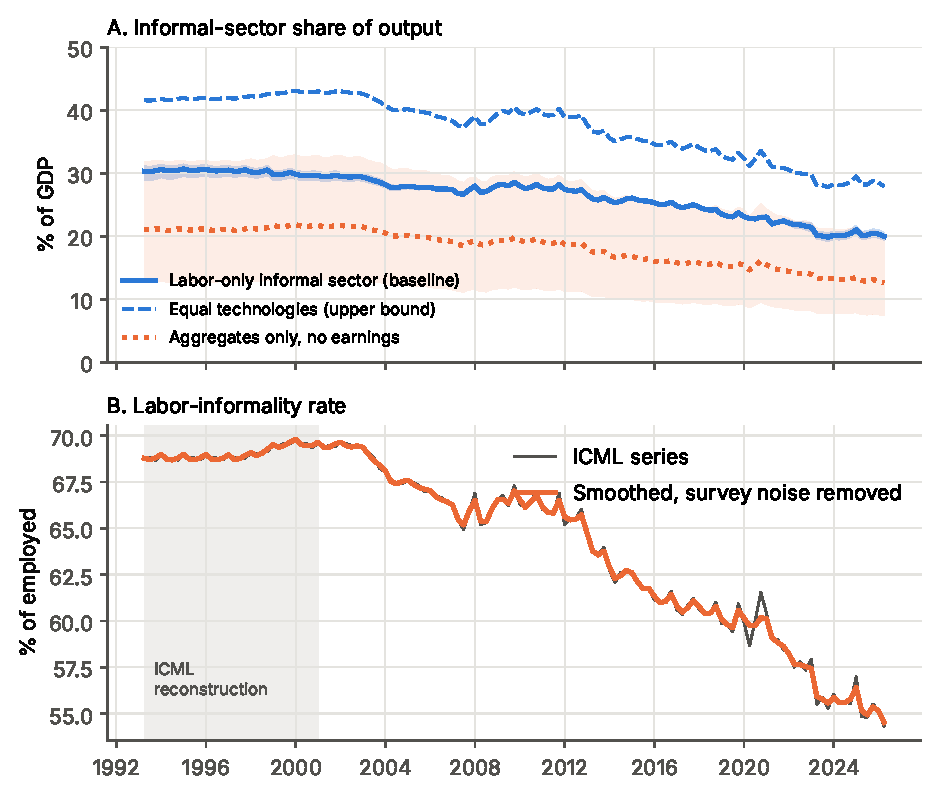
\includegraphics[width=0.9\textwidth]{fig_share_path.pdf}
\caption{Panel A: informal share of output, posterior median and 90\% band, baseline (labor-only informal sector, statutory non-wage costs), equal-technology estimate (upper bound) and estimate with aggregates only. Panel B: labor-informality rate from ICML and its smoothed value. The shaded area marks the ICML reconstruction (1993--2000).}
\label{fig:share}
\end{figure}

\subsection{Comparison with published estimates}
\label{sec:benchmarks}

Figure~\ref{fig:benchmarks} compares the estimate with the published annual series for Colombia included in our reference collection. Four families are available. The MIMIC estimates of Schneider and coauthors \citep{SchneiderBuehnMontenegro2010,MedinaSchneider2019} place the shadow economy at 36\%--40\% of official GDP in the 1990s and early 2000s and at 25\%--30\% after 2011. The enhanced MIMIC of \citet{AsllaniDellAnnoSchneider2024}, which restricts the concept to legal production deliberately concealed from the authorities, is almost flat at 24\%--27\%. The World Bank database \citep{ElginKoseOhnsorgeYu2021} reports a DGE series, built on the model of \citet{ElginOztunali2012}, that declines from 35\% in 1991 to 29\% in 2020, and a MIMIC series of 34\%--39\%. \citet{Vuletin2008} estimates 43.5\% for the early 2000s.

Published estimates differ among themselves by up to 19 percentage points in the same year, and the baseline lies inside that range throughout. It is 6 to 10 points below the MIMIC series of Schneider and coauthors between 1993 and 2005 and within about three points of \citet{MedinaSchneider2019} in 2008--2015, when that series falls to 25\%--31\%. It is within about one point of \citet{AsllaniDellAnnoSchneider2024} for 2009--2020, two to six points above it before and five below in 2021--2022. It is about six points below the World Bank DGE series in 2019--2020 and nine to fourteen below its MIMIC series. Its decline is steeper than that of the MIMIC series, which change little by construction. The equal-technology estimate lies at the top of the published range, next to \citet{Vuletin2008} and the World Bank MIMIC series, and the estimate without earnings below all of them.

\begin{figure}[H]
\centering
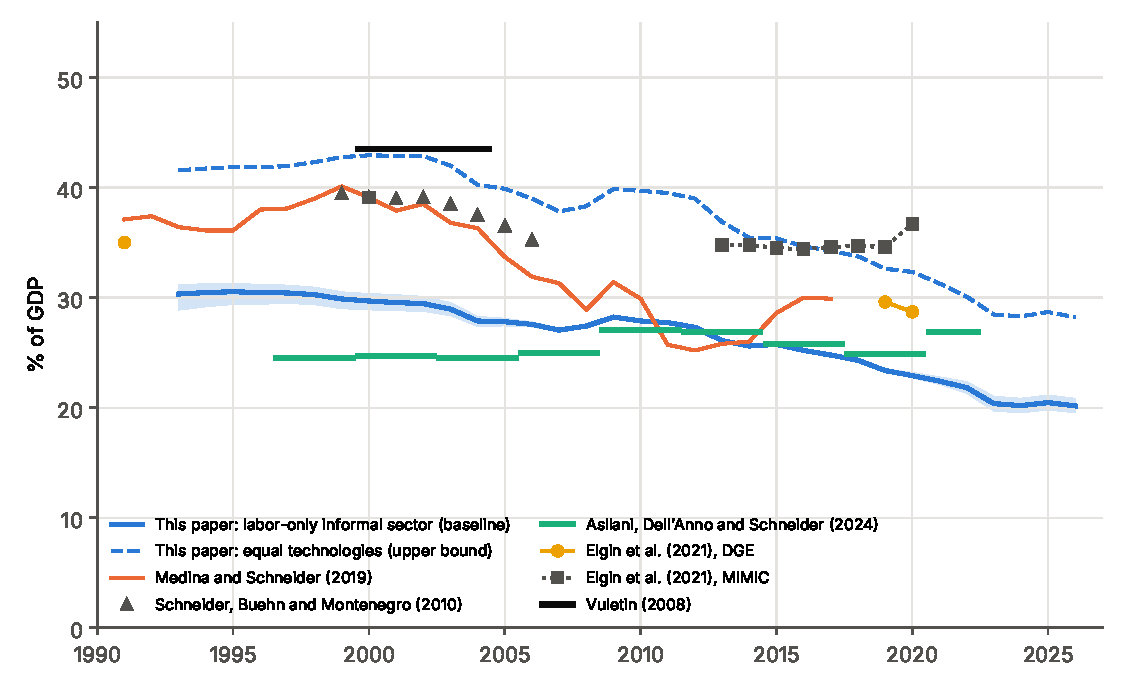
\includegraphics[width=0.9\textwidth]{fig_benchmarks.pdf}
\caption{Informal share of output: this paper and published estimates for Colombia (percent of GDP). Horizontal segments are period averages.}
\label{fig:benchmarks}
\end{figure}

Three differences in concept qualify the comparison. First, MIMIC estimates are expressed as a percentage of official GDP and treat the shadow economy as outside it, whereas the Colombian national accounts already include an estimate of the non-observed economy; our share is a fraction of measured GDP. Second, MIMIC levels are not independent measurements: they are converted to percentages of GDP with benchmark values from other studies, and \citet{AsllaniDellAnnoSchneider2024} anchor the scale to informal employment multiplied by an assumed informal wage, which is the accounting of Proposition~\ref{prop:share} with the earnings ratio assumed instead of measured. Third, our concept is the output of informal workers, which includes legal own-account production that is not concealed and excludes illegal activity. DANE's non-observed economy (22.4\% of gross production in the 2015 base) is not directly comparable either, because it refers to production rather than value added.

\subsection{Sensitivity}

The posterior bands reflect parameter and state uncertainty given the model and the measurement equation; uncertainty about the measurement assumptions is quantified by the sensitivity analysis. Table~\ref{tab:sensitivity} reports how the level changes with the concept of the formal wage (panel A), with other assumptions (panel B, around the constant-wedge specification) and with the technology (panel C). Three results stand out. First, the mapping from survey earnings to labor cost matters: with contributions only, the 2026 share is 22.8\% instead of 20.0\%, and with a constant 25\% wedge 20.6\%. Second, the capital share matters through the factor $1-\alpha$ in \eqref{eq:share}: with $\alpha=0.50$ the 2026 share is 17.0\% instead of 20.6\%. Third, the prior of $\eta$, the sample from 2007 and the capital--output ratio observed in levels leave the 2026 share within 0.2 points; observing capital raises the 1990s by about 3.5 points, because the model must accommodate the strong rise of the capital--output ratio in the sample. The equal-technology estimates bound the estimate from above.

\begin{table}[H]
\centering
\caption{Informal share of output under alternative specifications (posterior median and 90\% band, \%). $^{\dagger}$Largest $\hat R$ 1.053 (for $\theta$); the path is reported because it does not depend on $\theta$ (Table~\ref{tab:invariance}).}
\label{tab:sensitivity}
\scriptsize
\setlength{\tabcolsep}{4pt}
\begin{tabular}{l c c c c}
\toprule
\textbf{Specification} & $R$ & $\theta$ (steady state) & \textbf{1993Q2} & \textbf{2026Q2} \\
\midrule
\tableinput{tables/sensitivity.tex}
\bottomrule
\end{tabular}
\end{table}

The decline between 1993 and 2026, of ten to fifteen points, is common to every specification with earnings. Figure~\ref{fig:anchor} places the estimates on the mapping of Proposition~\ref{prop:share}.

\begin{figure}[H]
\centering
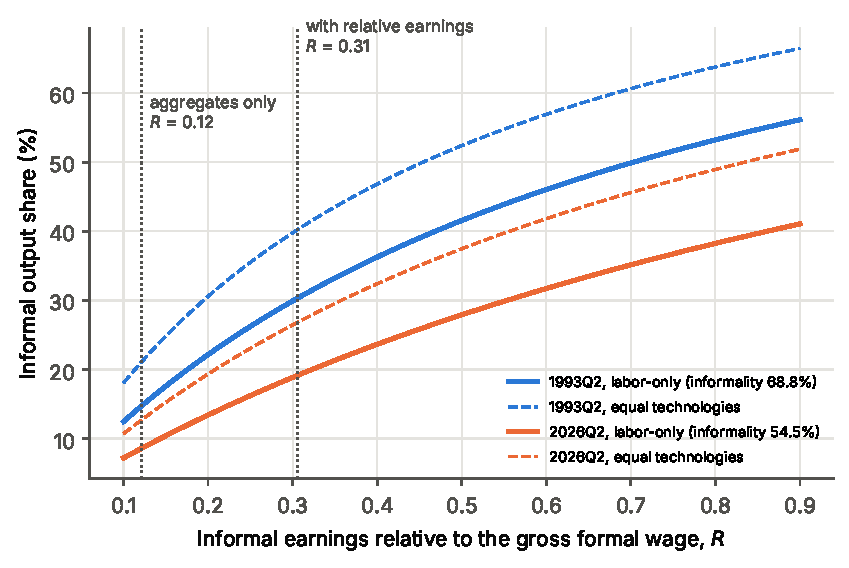
\includegraphics[width=0.75\textwidth]{fig_anchor_map.pdf}
\caption{Informal share of output implied by Proposition~\ref{prop:share} as a function of the earnings ratio $R$, at the informality rates of 1993Q2 and 2026Q2, for the labor-only and the equal-technology accounting. Dotted lines mark the posterior medians of $R$ with aggregates only and with the earnings observable.}
\label{fig:anchor}
\end{figure}
